\chapter{Wing Drag Characteristics}

\label{ch:workobject}
\markboth{Wing Drag Characteristics}{}

\begin{flushright}
	{\smaller
		\textit{It is not certain\\ that everything is uncertain}\\
		-- Blaise Pascal}
\end{flushright}


As mentioned in the previous chapter, the drag is the force component acting in the opposite direction to the airspeed vector.\\
There isn't a single classification of the drag but, dependent on the purpose of the work, the drag may be broken down in different way. Following will be explained the two main classifications.

\begin{itemize}
\item The drag is subdivided using a causal breakdown. In this way the drag contributes are in accordance with the physical mechanism such as the viscosity of the flow.
\item The drag is subdivided using a component breakdown. Every component of aircraft added an own drag contribute.
\end{itemize}

\begin{figure}[H]
\centering
{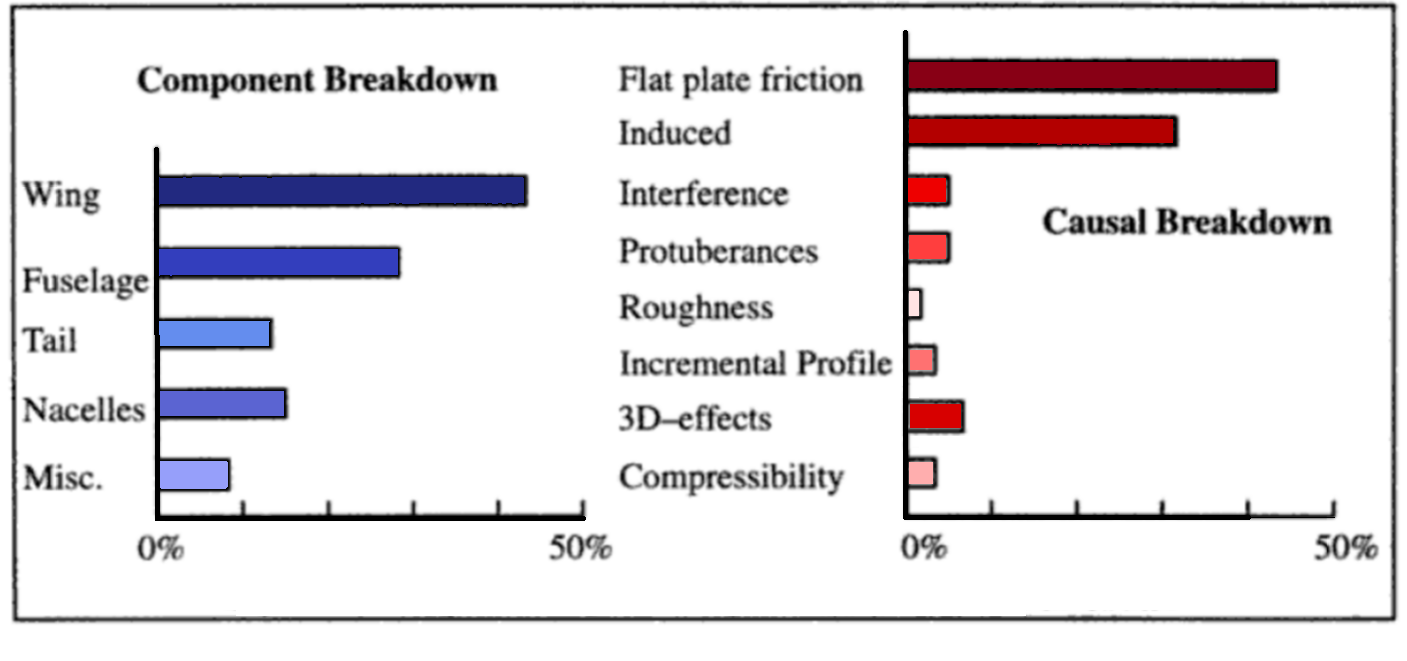
\includegraphics[height=6.4cm]{Immagini/component.png}} 
\caption{Drag breakdown for a business jet in cruise.}
\end{figure}

According to the casual breakdown it's possible to make a preliminary division considering normal and tangential stress. The tangential forces produce the {\bfseries friction drag}. While it's possible to divide the drag due of the normal component in viscous, that generates {\bfseries form drag}, and inviscid. A further division can be made for the last one, in {\bfseries induced drag}  and {\bfseries wave drag}.\\

\begin{figure}[H]
\centering
{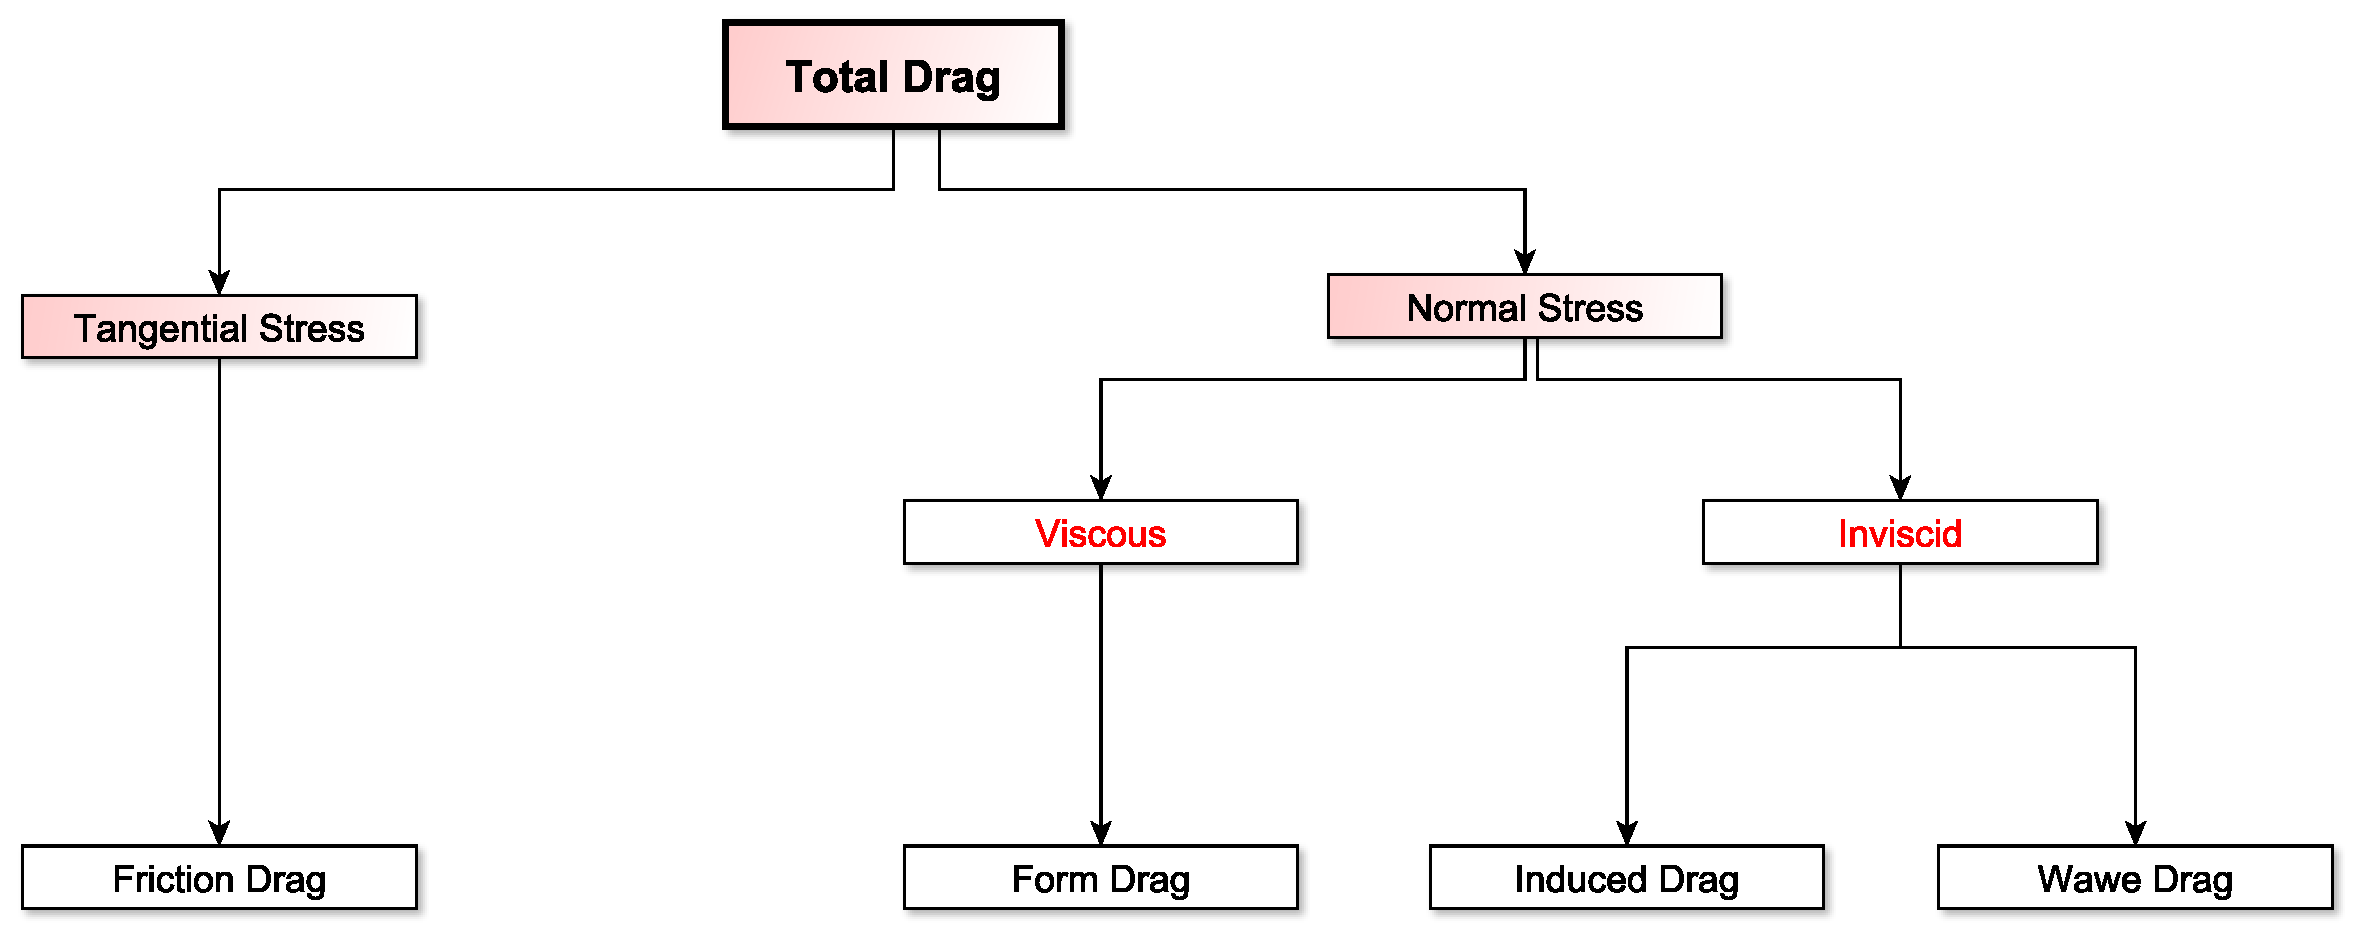
\includegraphics[height=6cm]{Immagini/dragcausal.pdf}} 
\caption{Causal breakdown of airplane drags.}
\end{figure}


Friction drag is caused by the air closest to the body’s surface that is dragged along with it. Due to this interaction shearing stresses are born within the thin layer of air (boundary layer) adiacent to the skin. The magnitude of this drag depends on the kind of boundary layer what can be laminar or turbulent in dependence on the Raynolds number. Usually it's accustomed to assume, at the flight speed and altitudes at which aircraft fly, a fully turbulent flow over the entire airplane. In this way a conservative result is obtained.\\
Form drag is caused by the air that is flowing over the body. The separation of air creates turbulence and results in pockets of low and high pressure that leave a wake behind the airplane. The departure of the boundary layer alters the pressure field from its inviscid distribution resulting in an additional drag component. The general size and shape of the body are the most important factors in form drag; bodies with a larger presented cross-section will have a higher drag than thinner bodies.\\
Induced drag is the drag due to lift. It is the drag created by the vortices at the tip of an aircraft's wing. The high pressure underneath the wing causes the airflow at the tips of the wings to curl around from bottom to top in a circular motion. So it's depend on the spanwise distribution of lift. \\
Wave drag is a component of the drag due to the presence of shock waves. Wave drag is independent of viscous effects, and tends to present itself as a sudden and dramatic increase in drag as the vehicle increases speed.
\\ \\ 
In this work the drag will be classified using a component breakdown. In this way it's possible to evaluate separately the wing drag and tail drag, considering the aerodynamic centers of these lifting surfaces as application point.

\begin{figure}[H]
\centering
{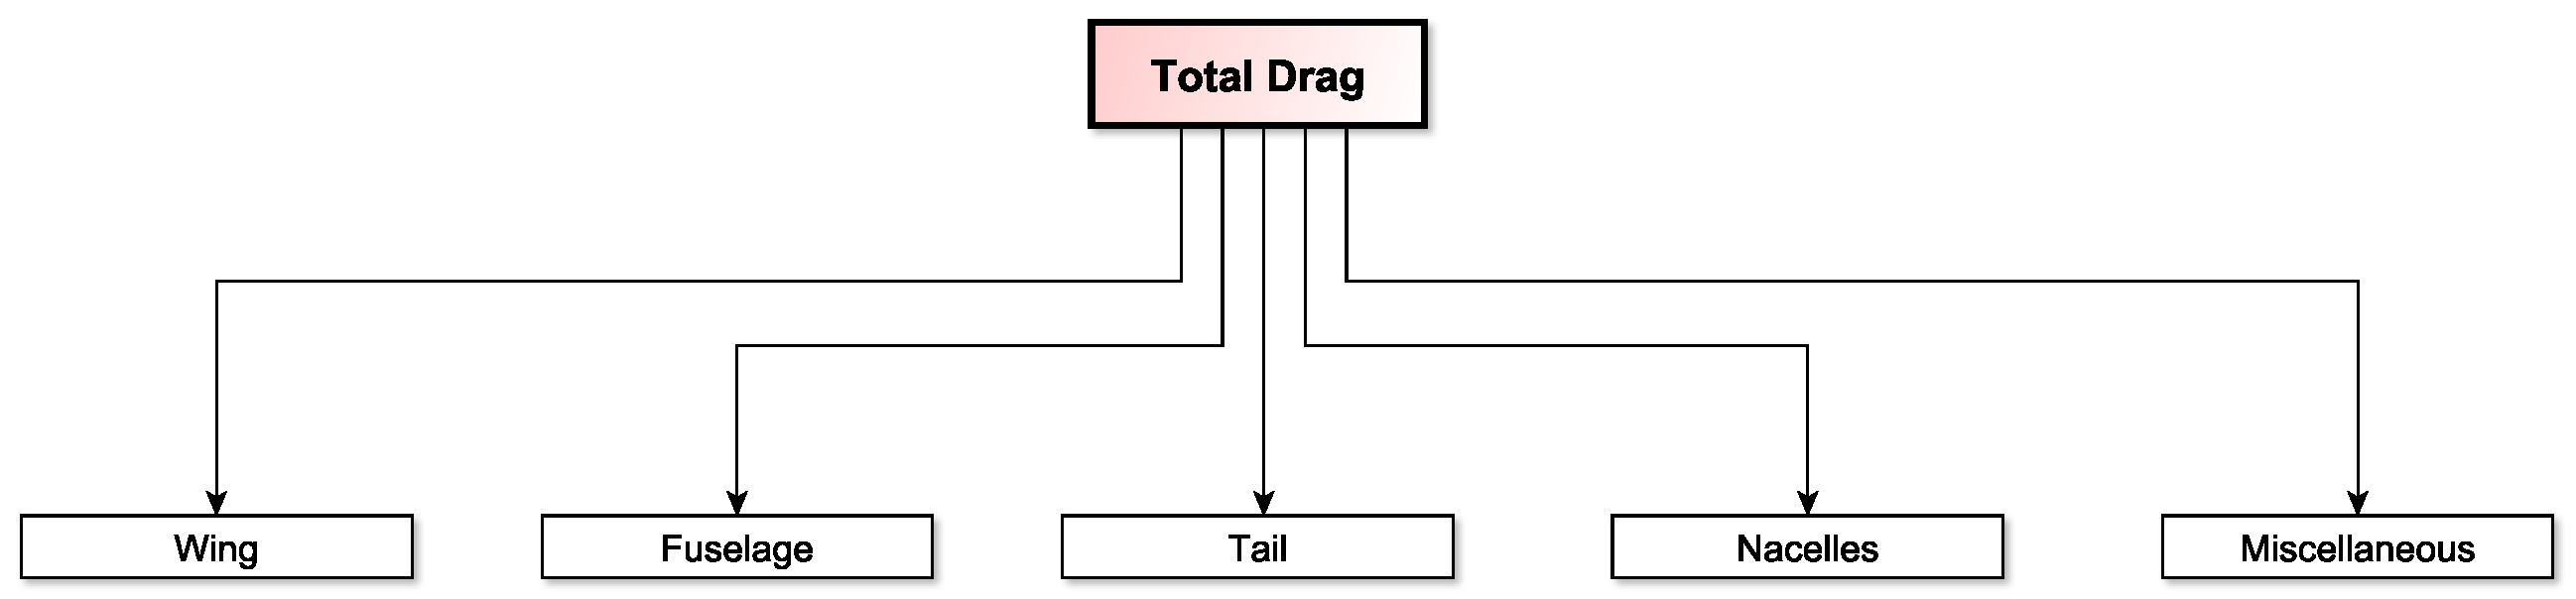
\includegraphics[height=3.6cm]{Immagini/dragco.pdf}} 
\caption{Components breakdown of airplane drags.}
\end{figure}

\section{Theoretical background}

In this thesis the drag coefficient of an isolated lifting surface is calculated starting from the load distribution and considering the parabolic approximation for the drag polar. The implemented process is the following:

\begin{enumerate}
\item First of all the load distribution at a given angle of attack has been calculated
\item Fifty points have been defined along the semispan
\item For each point, an intermediate profile is calculated
\item To each profile correspond the lift coefficient at that station
\item Starting from the CL, using a parabolic approximation for the drag polar, the CD is calculated with the following equation
\begin{equation}
CD = CD_{min} + (CL - CL_{CD_{min}})^2 + k
\end{equation}
\item Known the drag distribution it is possible to calculate the drag coefficient of the lifting surface integrating
\end{enumerate}

In the tool it is possible to choose the method used to calculate the load distribution. In particular it's possible to use Shrenk or Nasa-Blackwell method.\\

{\bfseries Schrenk Method} is based on an elliptical lifting coefficient distribution span wise hypothesis on the wing. This method also assumes that the pressure distribution is proportional to the wing area. \\ 

The {\bfseries Nasa-Blackwell} is a numerical method for calculating the subsonic load distribution for arbitrary lifting surface arrangements at a fixed angle of attack. The method is suitable for swept wings, non-planar wings, wing with pylons and/or end-plates; it can be also used to study the aerodynamic interaction of the wing and the horizontal tail. The method has been implemented because its results, as shown in the report, were in good agreement with the experimental results.
The lifting surfaces are divided in several rectangular horse-shoe vortices along the span; one horseshoe vortex along the chord is used, that is, the midpoints of the vortices are placed only at points along the quarter-chord lines. An equal number of control points are located along the three-quarter-chord lines. The velocity from the total vortex system is equated to the component of free-stream velocity normal to the lifting surface chord at each control point. Application of this tangent-flow boundary condition for a symmetrical loading provides a set of N simultaneous equations in the N unknown circulation strengths. Solution of this set of equations provides the loading distributions over the lifting surfaces. Mach number effect is introduced through a Prandtl-Glauert correction. Further details can be found in \cite{NASA:Blackwell}.


\section{Java Class Architecture}
In order to give more flexibility to the code, the calculation of drag coefficient is made from three different class summarized in the folloving table.

\begin{table}[H]
\begin{tabular}{p{7cm}p{7.5cm}}
\toprule
 \\[0.1	cm] 
\lstinline[language=Java]!integralFromCdAirfoil! & This method calculates the drag coefficient of the lifting surface using an integral and calling other method that fills the needed field. This is in the nested class \texttt{CalcCDAtAlpha}\\ \hline \\[0.1	cm] 
\lstinline[language=Java]!nasaBlackwell! &This method calculates drag distribution starting from the load distribution calculated with Nasa-Blackwell method and using a parabolic approximation for the drag polar.  This is in the nested class \texttt{CalcCdDistribution} \\ \hline \\ [0.1cm]
\lstinline[language=Java]!nasaBlackwell! & This method calculates the drag coefficient of an airfoil having the lift coefficient and using a parabolic approximation.\\ 
\bottomrule
\end{tabular}
\caption{Methods for drag coefficient calculatorof a lifting surface.}
\label{table:Table2}
\end{table}

% schema yed 

\section{Case Study}
% test class 
% output


